% Options for packages loaded elsewhere
\PassOptionsToPackage{unicode}{hyperref}
\PassOptionsToPackage{hyphens}{url}
\PassOptionsToPackage{dvipsnames,svgnames,x11names}{xcolor}
%
\documentclass[
  xelatex,
  ja=standard]{bxjsarticle}

\usepackage{amsmath,amssymb}
\usepackage{iftex}
\ifPDFTeX
  \usepackage[T1]{fontenc}
  \usepackage[utf8]{inputenc}
  \usepackage{textcomp} % provide euro and other symbols
\else % if luatex or xetex
  \usepackage{unicode-math}
  \defaultfontfeatures{Scale=MatchLowercase}
  \defaultfontfeatures[\rmfamily]{Ligatures=TeX,Scale=1}
\fi
\usepackage{lmodern}
\ifPDFTeX\else  
    % xetex/luatex font selection
  \setmainfont[BoldFont=Noto Sans CJK JP]{Noto Serif CJK JP}
\fi
% Use upquote if available, for straight quotes in verbatim environments
\IfFileExists{upquote.sty}{\usepackage{upquote}}{}
\IfFileExists{microtype.sty}{% use microtype if available
  \usepackage[]{microtype}
  \UseMicrotypeSet[protrusion]{basicmath} % disable protrusion for tt fonts
}{}
\makeatletter
\@ifundefined{KOMAClassName}{% if non-KOMA class
  \IfFileExists{parskip.sty}{%
    \usepackage{parskip}
  }{% else
    \setlength{\parindent}{0pt}
    \setlength{\parskip}{6pt plus 2pt minus 1pt}}
}{% if KOMA class
  \KOMAoptions{parskip=half}}
\makeatother
\usepackage{xcolor}
\setlength{\emergencystretch}{3em} % prevent overfull lines
\setcounter{secnumdepth}{5}
% Make \paragraph and \subparagraph free-standing
\ifx\paragraph\undefined\else
  \let\oldparagraph\paragraph
  \renewcommand{\paragraph}[1]{\oldparagraph{#1}\mbox{}}
\fi
\ifx\subparagraph\undefined\else
  \let\oldsubparagraph\subparagraph
  \renewcommand{\subparagraph}[1]{\oldsubparagraph{#1}\mbox{}}
\fi


\providecommand{\tightlist}{%
  \setlength{\itemsep}{0pt}\setlength{\parskip}{0pt}}\usepackage{longtable,booktabs,array}
\usepackage{calc} % for calculating minipage widths
% Correct order of tables after \paragraph or \subparagraph
\usepackage{etoolbox}
\makeatletter
\patchcmd\longtable{\par}{\if@noskipsec\mbox{}\fi\par}{}{}
\makeatother
% Allow footnotes in longtable head/foot
\IfFileExists{footnotehyper.sty}{\usepackage{footnotehyper}}{\usepackage{footnote}}
\makesavenoteenv{longtable}
\usepackage{graphicx}
\makeatletter
\def\maxwidth{\ifdim\Gin@nat@width>\linewidth\linewidth\else\Gin@nat@width\fi}
\def\maxheight{\ifdim\Gin@nat@height>\textheight\textheight\else\Gin@nat@height\fi}
\makeatother
% Scale images if necessary, so that they will not overflow the page
% margins by default, and it is still possible to overwrite the defaults
% using explicit options in \includegraphics[width, height, ...]{}
\setkeys{Gin}{width=\maxwidth,height=\maxheight,keepaspectratio}
% Set default figure placement to htbp
\makeatletter
\def\fps@figure{htbp}
\makeatother

\renewcommand{\thefootnote}{\arabic{footnote}}
\makeatletter
\makeatother
\makeatletter
\makeatother
\makeatletter
\@ifpackageloaded{caption}{}{\usepackage{caption}}
\AtBeginDocument{%
\ifdefined\contentsname
  \renewcommand*\contentsname{目次}
\else
  \newcommand\contentsname{目次}
\fi
\ifdefined\listfigurename
  \renewcommand*\listfigurename{図一覧}
\else
  \newcommand\listfigurename{図一覧}
\fi
\ifdefined\listtablename
  \renewcommand*\listtablename{表一覧}
\else
  \newcommand\listtablename{表一覧}
\fi
\ifdefined\figurename
  \renewcommand*\figurename{図}
\else
  \newcommand\figurename{図}
\fi
\ifdefined\tablename
  \renewcommand*\tablename{表}
\else
  \newcommand\tablename{表}
\fi
}
\@ifpackageloaded{float}{}{\usepackage{float}}
\floatstyle{ruled}
\@ifundefined{c@chapter}{\newfloat{codelisting}{h}{lop}}{\newfloat{codelisting}{h}{lop}[chapter]}
\floatname{codelisting}{コード}
\newcommand*\listoflistings{\listof{codelisting}{コード一覧}}
\makeatother
\makeatletter
\@ifpackageloaded{caption}{}{\usepackage{caption}}
\@ifpackageloaded{subcaption}{}{\usepackage{subcaption}}
\makeatother
\makeatletter
\@ifpackageloaded{tcolorbox}{}{\usepackage[skins,breakable]{tcolorbox}}
\makeatother
\makeatletter
\@ifundefined{shadecolor}{\definecolor{shadecolor}{rgb}{.97, .97, .97}}
\makeatother
\makeatletter
\makeatother
\makeatletter
\makeatother
\ifLuaTeX
\usepackage[bidi=basic]{babel}
\else
\usepackage[bidi=default]{babel}
\fi
\babelprovide[main,import]{japanese}
% get rid of language-specific shorthands (see #6817):
\let\LanguageShortHands\languageshorthands
\def\languageshorthands#1{}
\ifLuaTeX
  \usepackage{selnolig}  % disable illegal ligatures
\fi
\usepackage[]{natbib}
\bibliographystyle{jecon}
\IfFileExists{bookmark.sty}{\usepackage{bookmark}}{\usepackage{hyperref}}
\IfFileExists{xurl.sty}{\usepackage{xurl}}{} % add URL line breaks if available
\urlstyle{same} % disable monospaced font for URLs
\hypersetup{
  pdftitle={経済成長},
  pdfauthor={土井翔平},
  pdflang={ja},
  colorlinks=true,
  linkcolor={NavyBlue},
  filecolor={Maroon},
  citecolor={NavyBlue},
  urlcolor={NavyBlue},
  pdfcreator={LaTeX via pandoc}}

\title{経済成長}
\usepackage{etoolbox}
\makeatletter
\providecommand{\subtitle}[1]{% add subtitle to \maketitle
  \apptocmd{\@title}{\par {\large #1 \par}}{}{}
}
\makeatother
\subtitle{国際公共政策学}
\author{土井翔平}
\date{2023-07-11}

\begin{document}
\maketitle
\ifdefined\Shaded\renewenvironment{Shaded}{\begin{tcolorbox}[breakable, interior hidden, borderline west={3pt}{0pt}{shadecolor}, enhanced, boxrule=0pt, frame hidden, sharp corners]}{\end{tcolorbox}}\fi

\hypertarget{ux306fux3058ux3081ux306b}{%
\section*{はじめに}\label{ux306fux3058ux3081ux306b}}
\addcontentsline{toc}{section}{はじめに}

\begin{itemize}
\tightlist
\item
  政治は経済成長に影響するのか?
\item
  なぜ国ごとに経済的豊かさが異なるのか?
\item
  経済成長と不平等の縮小は両立するのか?
\end{itemize}

\begin{figure}[htpb]

{\centering \includegraphics[width=0.8\textwidth,height=\textheight]{figures/gdp-per-capita-maddison-2018.png}

}

\caption{一人あたりGDPの長期的変化}

\end{figure}

\begin{figure}[htpb]

{\centering \includegraphics[width=0.8\textwidth,height=\textheight]{figures/income_group.png}

}

\caption{各国の所得水準}

\end{figure}

\begin{figure}[htpb]

{\centering \includegraphics[width=0.8\textwidth,height=\textheight]{figures/u-shape.png}

}

\caption{経済的不平等の推移}

\end{figure}

\begin{figure}[htpb]

{\centering \includegraphics[width=0.8\textwidth,height=\textheight]{figures/l-shape.png}

}

\caption{経済的不平等の推移}

\end{figure}

\hypertarget{ux7d4cux6e08ux6210ux9577ux3068ux56fdux5185ux653fux6cbb}{%
\section{経済成長と国内政治}\label{ux7d4cux6e08ux6210ux9577ux3068ux56fdux5185ux653fux6cbb}}

\hypertarget{ux653fux6cbbux4f53ux5236}{%
\subsection{政治体制}\label{ux653fux6cbbux4f53ux5236}}

\begin{figure}[htpb]

{\centering 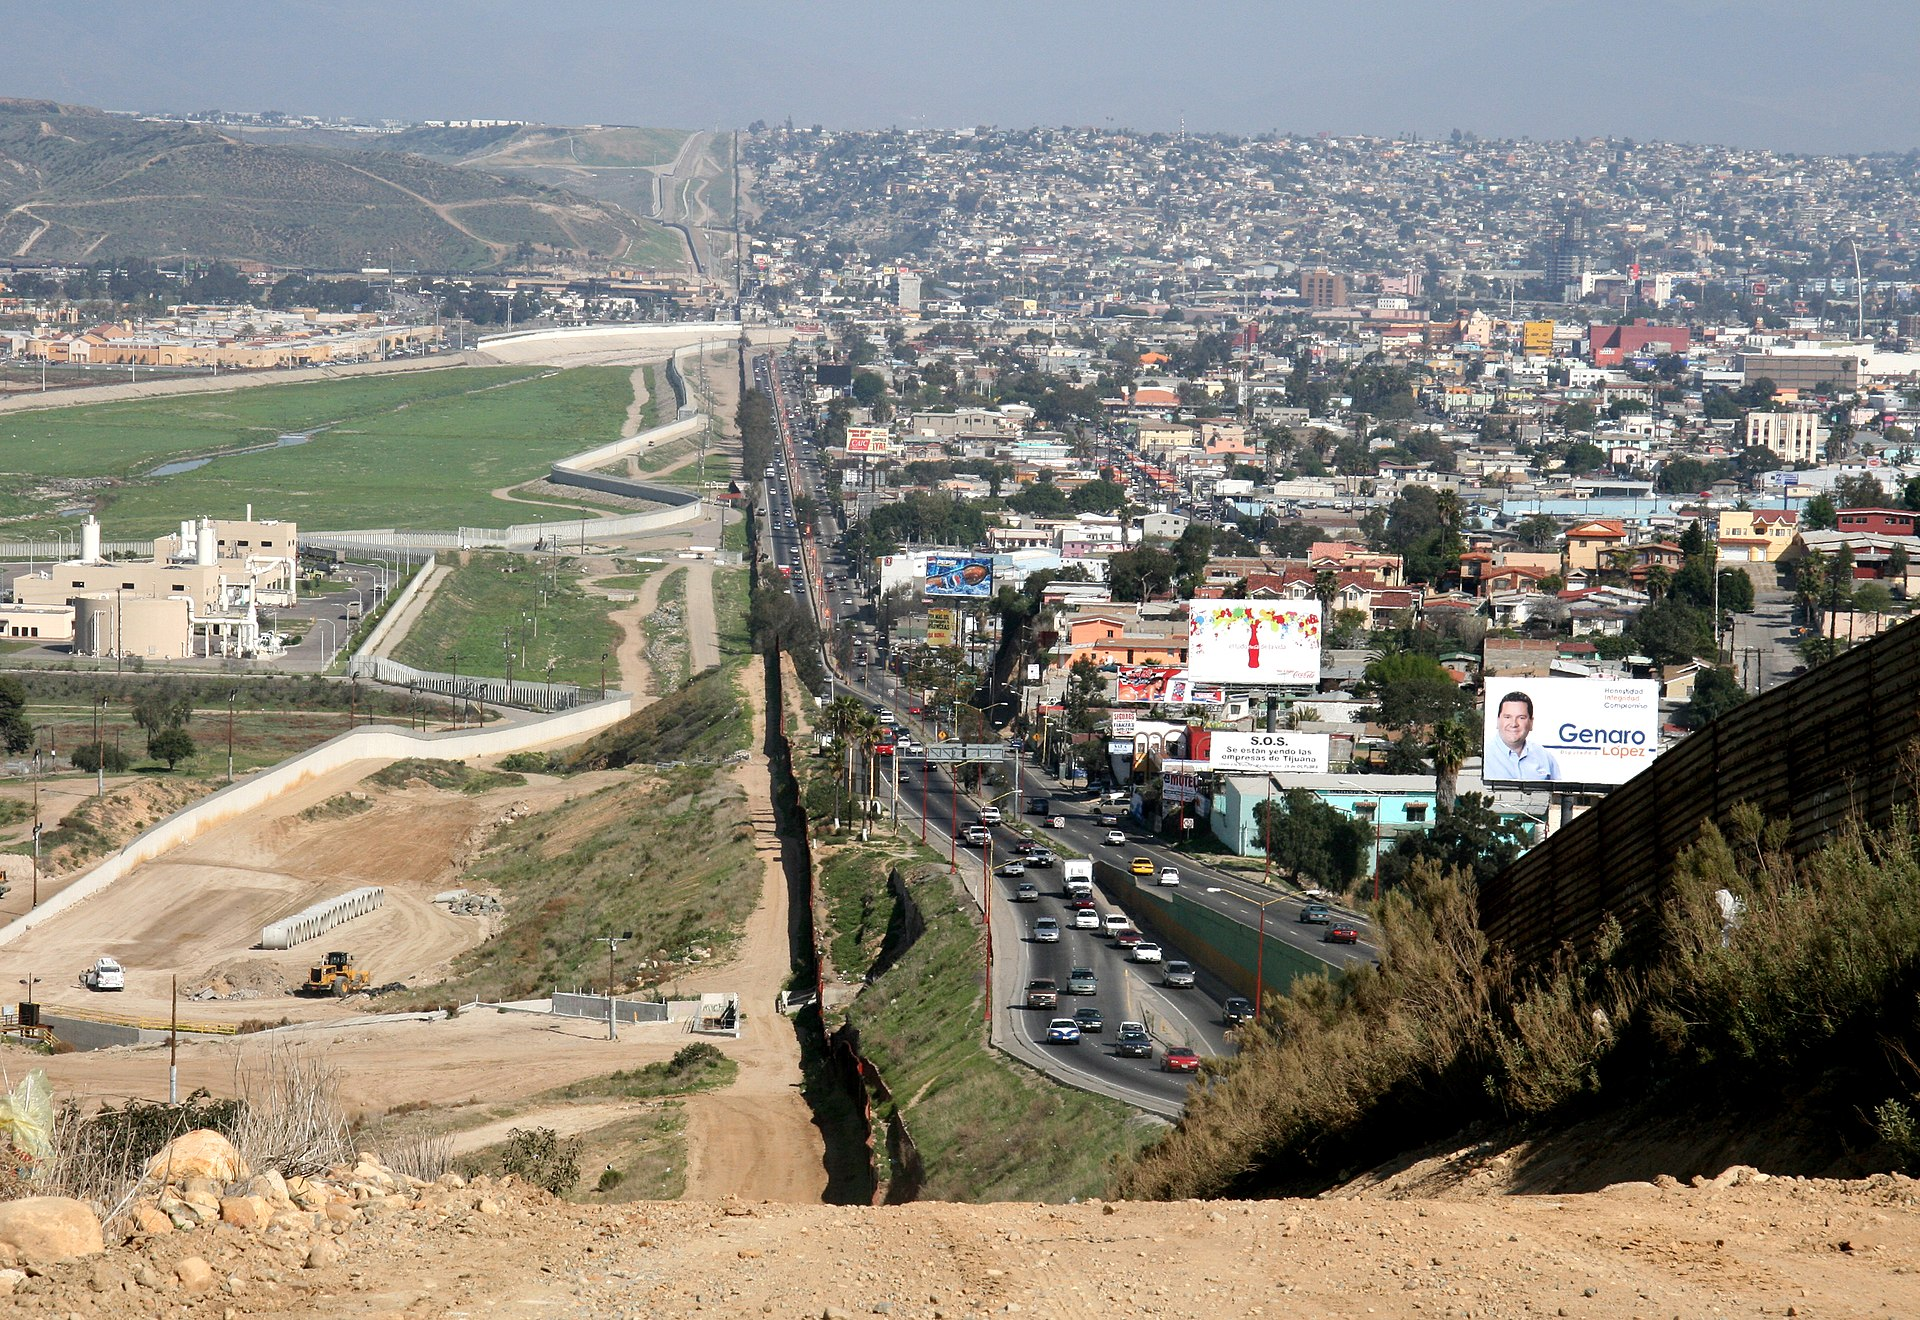
\includegraphics[width=0.8\textwidth,height=\textheight]{figures/Border_USA_Mexico.jpg}

}

\caption{アメリカとメキシコの国境}

\end{figure}

世界全体で見ると経済成長/経済成長をしている国もいれば、そうでない国も

\begin{itemize}
\tightlist
\item
  韓国や台湾は工業化に成功して経済成長
\item
  サブサハラ・アフリカを中心に経済が停滞
\end{itemize}

地理(特に気候)や人種の違いが経済発展の違いを生む?

\begin{itemize}
\tightlist
\item
  ほとんど同じような地域(したがって地理的条件や人種構成も似ているはず)\(\leadsto\)全く異なる経済発展
\end{itemize}

\(\leadsto\)国家の違い、特に政治体制の違いが重要\citep{robinson2006}

政府は\textbf{インフラ}を供給&\textbf{所有権}を保障\(\leadsto\)経済成長を促進

\begin{itemize}
\tightlist
\item
  インフラ:交通インフラ、公衆衛生や教育といった社会的インフラ
\item
  所有権を保障\(\leadsto\)市民は安心して経済活動(特に投資)に専念
\end{itemize}

政府にとっても経済成長することは望ましい/なぜそのような政策を実行できないのか?

\begin{itemize}
\tightlist
\item
  大地主や大企業、都市部のエリートなど政権運営に必要な勢力の利益になるような政策(インフラ投資への反対、農民への課税や補助金)を行い、多数派の利益を損なう。
\item
  民族対立がある場合\citep{alesina2005}や権威主義体制である場合\citep{baum2003, stasavage2005, brown2009}は経済成長が難しい。
\end{itemize}

\begin{figure}[htpb]

{\centering 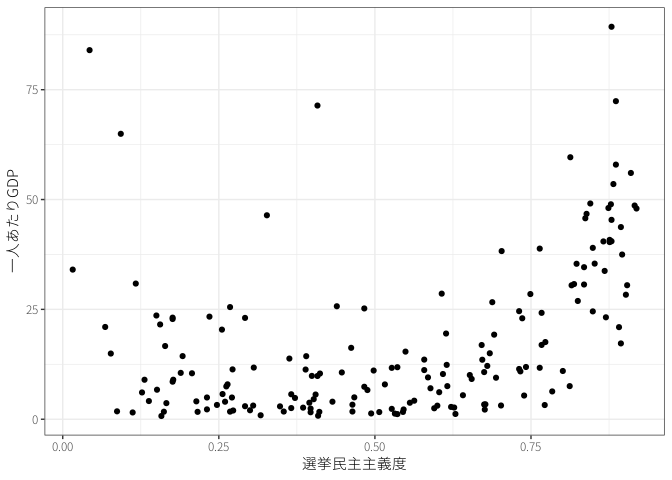
\includegraphics{economic_development_files/figure-pdf/unnamed-chunk-2-1.png}

}

\caption{民主主義と経済水準}

\end{figure}

\hypertarget{ux8cc7ux6e90ux306eux546aux3044}{%
\subsubsection{資源の呪い}\label{ux8cc7ux6e90ux306eux546aux3044}}

\textbf{資源の呪い} (resource
curse):農産物や資源が豊富な国では経済成長がしにい&民主的な政治体制ができにくい現象\citep{ross1999, mehlum2006, ross2015}

\begin{itemize}
\tightlist
\item
  経済成長ためのインフラ投資をする必要がない。
\item
  大地主や大企業に権力が集中する政治体制を構築
\end{itemize}

逆説的に、資源の乏しい国では経済活動を活発化させるためにインフラ投資や民主化を行う。

\begin{figure}[htpb]

{\centering 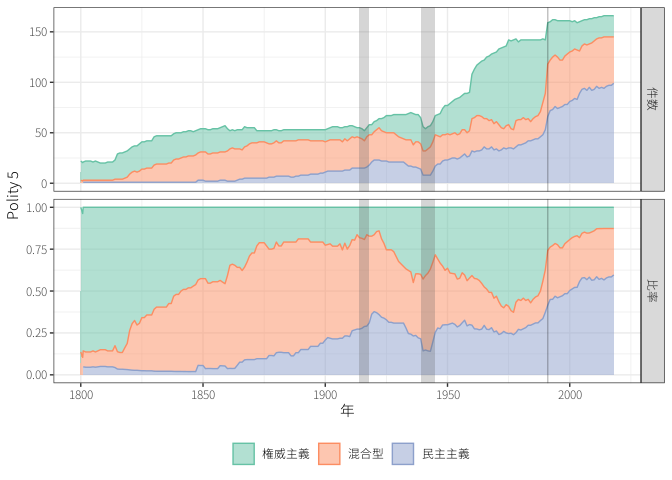
\includegraphics{economic_development_files/figure-pdf/unnamed-chunk-3-1.png}

}

\caption{天然資源と政治体制}

\end{figure}

\hypertarget{ux690dux6c11ux5730ux652fux914d}{%
\subsubsection{植民地支配}\label{ux690dux6c11ux5730ux652fux914d}}

植民地支配\(\leadsto\)政治体制

\begin{itemize}
\tightlist
\item
  大航海時代においてポルトガルやスペインは先に資源の豊富な南米/後発のイギリスやフランスは資源の乏しい北米に進出
\item
  南米ではプランテーションなど搾取的な体制が成立/北米では民主的な体制が成立\(\leadsto\)その後の経済発展\citep{engerman2000, acemoglu2016}
\end{itemize}

北米に比べて熱帯病などで死亡率の高かった南米では移住が困難\(\leadsto\)原住民から資源を搾取する体制が構築\(\leadsto\)現代の低成長\citep{acemoglu2001}

\begin{figure}[htpb]

{\centering 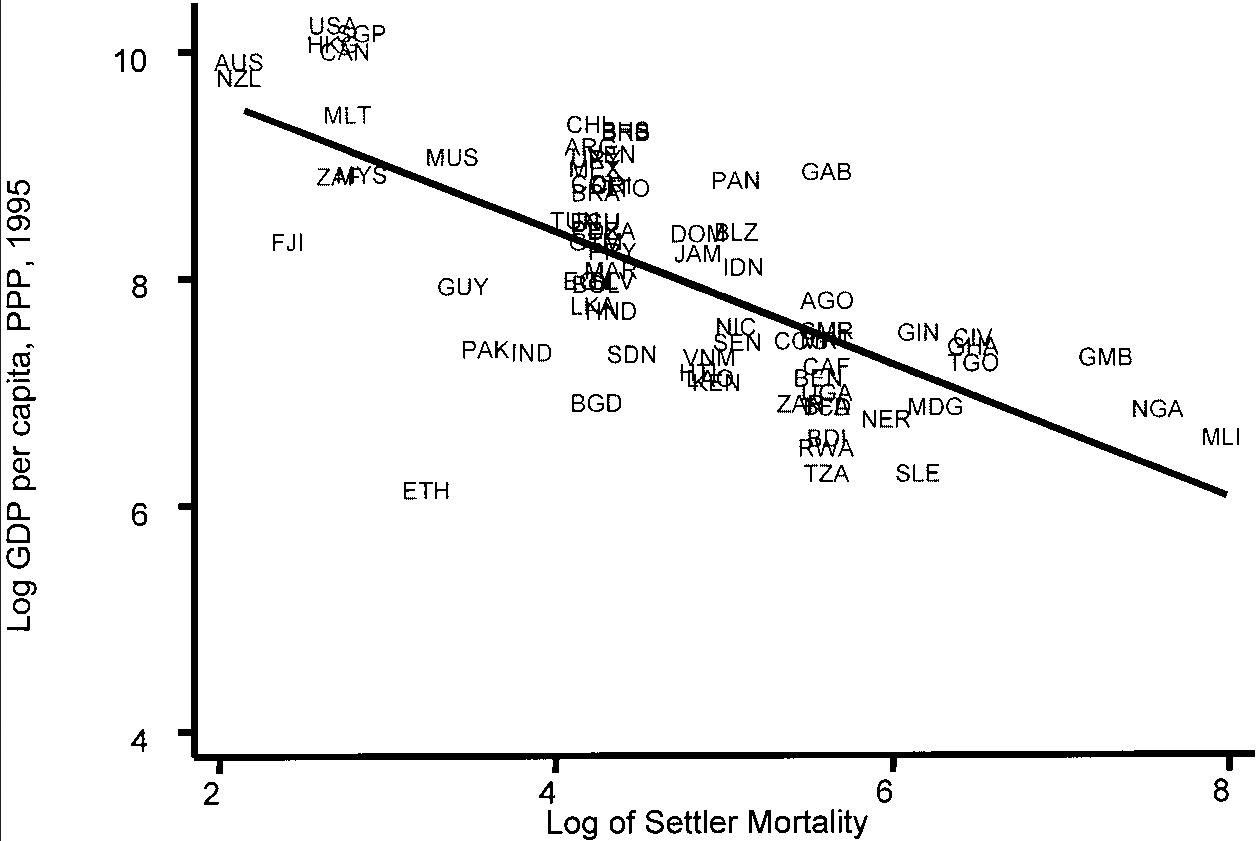
\includegraphics{figures/acemoglu1.png}

}

\caption{\citet{acemoglu2001}}

\end{figure}

\begin{figure}[htpb]

{\centering 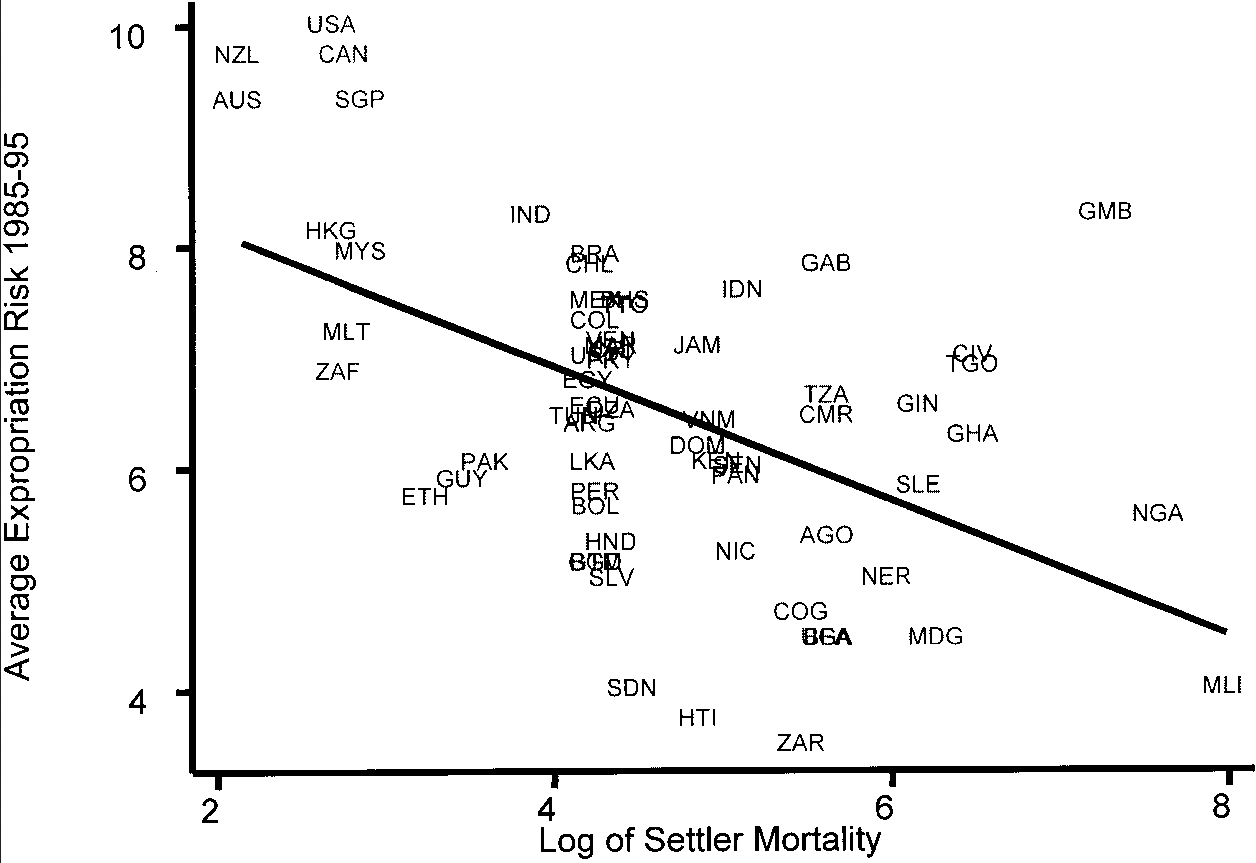
\includegraphics{figures/acemoglu2.png}

}

\caption{\citet{acemoglu2001}}

\end{figure}

植民地時代の死亡率が直接的に現代の経済水準に影響を与えているとは考えにくい\(\leadsto\)政治体制が経済成長に影響を及ぼしている

\hypertarget{ux958bux767aux653fux7b56}{%
\subsection{開発政策}\label{ux958bux767aux653fux7b56}}

\hypertarget{ux8f38ux5165ux4ee3ux66ffux5de5ux696dux5316}{%
\subsubsection{輸入代替工業化}\label{ux8f38ux5165ux4ee3ux66ffux5de5ux696dux5316}}

一般的に自由貿易は先進国と途上国のどちらにも恩恵をもたらすものだと考えられる

\(\leadsto\)\textbf{従属理論} (dependency
theory):途上国は自由貿易によって搾取されているという考え(1950年代ごろ)

\begin{itemize}
\tightlist
\item
  多くの後発開発途上国は農産品や資源、原材料など\textbf{一次産品}
  (primary goods) を輸出
\item
  一次産品は生産者が非常に多い\(\leadsto\)市場原理によって価格が定まる

  \begin{itemize}
  \tightlist
  \item
    長期的に見て下降傾向にある
  \end{itemize}
\item
  先進国の生産する工業製品は生産者の数が少ない\textbf{寡占} (oligopoly)
  状態\(\leadsto\)企業に価格決定力
\end{itemize}

\(\leadsto\)先進国は有利な\textbf{交易条件} (terms of trade) の下で貿易

\(\leadsto\)経済成長(特に工業化)の戦略の一つとして\textbf{輸入代替工業化}
(import-substituting industrialization)

\begin{itemize}
\tightlist
\item
  工業製品の輸入を制限し、自国内で製造できるようにする\(\leadsto\)工業化
\item
  政府は国営企業によってインフラを安価に供給し、補助金や減税、低金利ローンなどによって国内産業を優遇
\item
  工業化には成功する/市場原理に反して産業を保護\(\leadsto\)国際競争力が高まらず、輸出できないという問題
\end{itemize}

\hypertarget{ux8f38ux51faux5fd7ux5411ux5de5ux696dux5316}{%
\subsubsection{輸出志向工業化}\label{ux8f38ux51faux5fd7ux5411ux5de5ux696dux5316}}

1960年代、Four Asian
Tigersと呼ばれる韓国、台湾、シンガポール、香港は\textbf{輸出志向型工業化}
(export-oriented industrialization) を採用

\begin{itemize}
\tightlist
\item
  低金利ローンや減税、通貨安への誘導などを通じて輸出を振興
\item
  これらの国や地域は急速な工業化と経済成長を達成\(\leadsto\)\textbf{東アジアの奇跡}
\end{itemize}

1980年代に南米などで債務危機\(\leadsto\)輸入代替工業化を採用している国は、返済のための外貨を獲得することが困難

\begin{itemize}
\tightlist
\item
  債務返済のために\textbf{国際通貨基金} (International Monetary Fund:
  IMF)
  から融資や債務削減を受ける\(\leadsto\)自由経済に合致するコンディショナリティを受け入れ
\end{itemize}

輸出志向型工業化を採用していた国も債務危機の影響を受けた/輸出によって外貨を獲得し、経済を回復

\(\leadsto\)冷戦の終結も相まって、1990年ごろにはほとんどの開発途上国が輸入代替工業化を放棄して、世界経済との繋がりを構築

\hypertarget{ux7d4cux6e08ux6210ux9577ux3068ux56fdux969bux95a2ux4fc2}{%
\section{経済成長と国際関係}\label{ux7d4cux6e08ux6210ux9577ux3068ux56fdux969bux95a2ux4fc2}}

現代のグローバル化の特徴の一つは資本の越境的な (transnational)
移動の拡大

\begin{itemize}
\tightlist
\item
  通貨:自国通貨と他国通貨の交換(為替)
\item
  投資

  \begin{itemize}
  \tightlist
  \item
    融資:外国企業への融資、外国国債の購入
  \item
    直接投資:外国における企業や向上の設置
  \item
    間接投資:外国企業の株式の購入
  \end{itemize}
\item
  援助:先進国による途上国の支援
\end{itemize}

\hypertarget{ux901aux8ca8}{%
\subsection{通貨}\label{ux901aux8ca8}}

\textbf{為替} (exchange):自国通貨で外国通貨を購入すること

\begin{itemize}
\tightlist
\item
  為替の際の交換比率のことを\textbf{為替レート}と呼ぶ。

  \begin{itemize}
  \tightlist
  \item
    例えば、\href{https://info.finance.yahoo.co.jp/fx/convert/}{1USドルは140円}と交換できる。
  \item
    言い換えれば、1USドルの値段は(日本円にして)140円である。
  \end{itemize}
\end{itemize}

自国通貨の価値が高く(低く)なる\(\leadsto\)多くの(少ない)外国通貨を購入

\begin{itemize}
\tightlist
\item
  1USドルが130円になると\textbf{円高}
\item
  1USドルが150円になると\textbf{円安}
\end{itemize}

\hypertarget{ux901aux8ca8ux306eux4fa1ux5024}{%
\subsubsection{通貨の価値}\label{ux901aux8ca8ux306eux4fa1ux5024}}

\begin{figure}[htpb]

{\centering \includegraphics{economic_development_files/mediabag/1280px-Exchange_rate.png}

}

\caption{\href{https://commons.wikimedia.org/wiki/File:Exchange_rate_arrangements_map.svg}{為替制度}}

\end{figure}

\textbf{固定相場制} (fixed exchange):為替レートを一定に固定する場合

\begin{itemize}
\tightlist
\item
  例:金本位制
\end{itemize}

\textbf{変動相場制} (floating exchange):為替レートを市場に委ねる場合

\(\leadsto\)変動相場制の下では需要と供給の法則に従って価格が決定

\begin{enumerate}
\def\labelenumi{\arabic{enumi}.}
\tightlist
\item
  \textbf{購買力平価}:物価に基づいて為替レートが決定

  \begin{itemize}
  \tightlist
  \item
    日本が輸出\(\leadsto\)日本円の需要が高まる\(\leadsto\)円高
  \end{itemize}
\item
  \textbf{金利平価}:金利に基づいて為替レートが決定

  \begin{itemize}
  \tightlist
  \item
    アメリカの金利が上がる\(\leadsto\)USドルの需要が高まる\(\leadsto\)円安
  \end{itemize}
\end{enumerate}

中央銀行は\textbf{外貨準備}を用いて、為替レートの安定化のために\textbf{為替介入}を行うことがある。

\hypertarget{ux8fd1ux96a3ux7aaeux4e4fux5316ux653fux7b56}{%
\subsubsection{近隣窮乏化政策}\label{ux8fd1ux96a3ux7aaeux4e4fux5316ux653fux7b56}}

外国製品を輸入する場合は自国通貨で外国通貨を購入しなくてはいけない

\(\leadsto\)為替レートと貿易は密接な関係にある。

\begin{longtable}[]{@{}lcc@{}}
\toprule\noalign{}
& 輸出 & 輸入 \\
\midrule\noalign{}
\endhead
\bottomrule\noalign{}
\endlastfoot
自国通貨が高くなる & 減少 & 増加 \\
自国通貨が安くなる & 増加 & 減少 \\
\end{longtable}

\begin{itemize}
\tightlist
\item
  例えば、480万円の車は1USドル110円なら約4.4万USドルで売れるが、120円(円安)だと4万USドル、100円(円高)だと4.8万USドルで売れる。
\end{itemize}

各国は通貨を切り下げることで輸出を促進

\begin{itemize}
\tightlist
\item
  しかし、他国に経済的負担を押し付ける\textbf{近隣窮乏化政策} (beggar
  thy neighbour) となる。
\end{itemize}

\(\leadsto\)通貨切り下げ競争は囚人のジレンマの構造

\hypertarget{ux56fdux969bux901aux8ca8ux4f53ux5236}{%
\subsubsection{国際通貨体制}\label{ux56fdux969bux901aux8ca8ux4f53ux5236}}

金ドル本位制やドル基軸通貨体制:USドルと金の交換レートを保証し、各国は自国通貨とUSドルの為替レートを一定の範囲内に収める調整可能な固定相場制

\begin{itemize}
\tightlist
\item
  各国は輸入による金の流出を恐れる必要がなし
\item
  USドルを\textbf{基軸通貨}として受け入れる必要

  \begin{itemize}
  \tightlist
  \item
    アメリカの圧倒的経済力を背景に金との交換を保証
  \item
    アメリカが輸入をする(貿易赤字を引き受ける)ことでUSドルを世界に供給
  \end{itemize}
\end{itemize}

\textbf{国際通貨基金} (International Monetary Fund: IMF)
はブレトン・ウッズ体制を支える機関として設立

\begin{itemize}
\tightlist
\item
  外貨準備が不足して固定相場を維持できない国を短期的に融資

  \begin{itemize}
  \tightlist
  \item
    \textbf{コンディショナリティ}:融資の際の条件
  \end{itemize}
\end{itemize}

USドルの供給が増える(ドル過剰)\(\leadsto\)アメリカの金準備が足りなくなる?

\(\leadsto\)\textbf{流動性のジレンマ}:ドルの供給によってドルの価値が信頼されなくなる

\textbf{ニクソン・ショック}:1971年、貿易赤字に不満を持っていたアメリカはUSドルと金の交換を停止

\(\leadsto\) 1973年に先進国は変動相場制に移行し、資本の移動を自由化

変動相場制のもとでは為替レートの変動が激しいときも\(\leadsto\)\textbf{政策協調}によって安定化

\begin{itemize}
\tightlist
\item
  1985年の\textbf{プラザ合意}ではアメリカの貿易赤字を減らすためにドル安介入
\item
  円高による不況を回避するための金融政策\(\leadsto\)金利が低下\(\leadsto\)\textbf{バブル経済}が発生
\end{itemize}

\hypertarget{ux50b5ux52d9ux5371ux6a5f}{%
\subsection{債務危機}\label{ux50b5ux52d9ux5371ux6a5f}}

貿易に加えて国際的な投資も経済成長にとって重要な役割

\(\leadsto\)政府は\textbf{国債} (sovereign bond)
を発行し、資金を調達することで増税せずに財政支出を拡大

\begin{itemize}
\tightlist
\item
  ヘクシャー=オーリン・モデルと同様、資本の潤沢な先進国の投資家は金利の高い途上国に融資をすることで利潤を拡大
\end{itemize}

財政支出が失敗し、税収が上がらず、債務の履行が困難\(\leadsto\)債務危機

\begin{itemize}
\tightlist
\item
  債務国は\textbf{緊縮財政} (austerity)
  によって支出を削減し、税収によって債務を返済する/\textbf{デフォルト}によって債務の履行を拒否する
\item
  債権国はできる限り債務を返還してほしい/デフォルトされることで国内の金融機関へ影響が波及するのを恐れて、救済
  (bailout) する
\end{itemize}

\(\leadsto\)債務国も債権国もデフォルトすることは避けたいが、できる限り少なく(多く)返済したい(回収したい)ため、交渉問題に

\hypertarget{ux56fdux969bux901aux8ca8ux57faux91d1}{%
\subsubsection{国際通貨基金}\label{ux56fdux969bux901aux8ca8ux57faux91d1}}

\textbf{国際通貨基金} (International Monetary Fund: IMF)
:約1兆USドルの融資能力を持つ世界最大の貸し手

\begin{itemize}
\tightlist
\item
  IMFでは経済水準を元に算出される出資額、\href{https://www.mof.go.jp/policy/international_policy/imf/gaiyou.htm}{\textbf{クォータ}}に比例して投票権が配分
\item
  IMFにおける多くの決定には85\%以上の賛成が必要\(\leadsto\)アメリカや欧州連合は事実上の拒否権
\end{itemize}

\begin{figure}[htpb]

{\centering 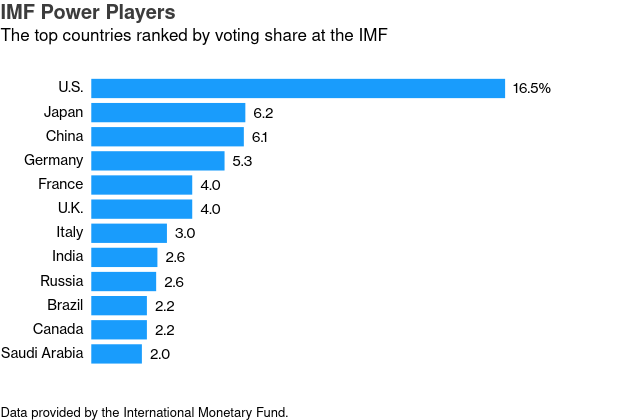
\includegraphics{figures/imf_vote.png}

}

\caption{\href{https://www.bloomberg.co.jp/news/articles/2021-10-11/R0U4IBDWLU6A01}{国際通貨基金における投票権}}

\end{figure}

\(\leadsto\)IMFからのコンディショナリティを受け入れることで低金利の融資を得る。

\begin{itemize}
\tightlist
\item
  市場からはIMFの基準に従った政策をしているという評判
\item
  緊縮財政や規制緩和はしばしば債務国の経済状況を悪化
\end{itemize}

\hypertarget{ux50b5ux52d9ux306eux7f60}{%
\subsubsection{債務の罠}\label{ux50b5ux52d9ux306eux7f60}}

\textbf{債務の罠} (debt trap
diplomacy):過度な融資をすることで債務の返済を困難にさせ、代わりにインフラの使用権などを要求する

\begin{itemize}
\tightlist
\item
  中国の\textbf{一帯一路} (Belt and Road Initiative: BRI)
  は債務の罠ではないかと先進国は批判
\end{itemize}

\hypertarget{ux591aux56fdux7c4dux4f01ux696d}{%
\subsection{多国籍企業}\label{ux591aux56fdux7c4dux4f01ux696d}}

国債の購入以外に、\textbf{対外直接投資} (foreign direct investment: FDI)
も主要な国際的投資の一種

\begin{itemize}
\tightlist
\item
  外国企業の買収や海外における工場の建設など、直接的に管理を行う投資
\end{itemize}

\textbf{多国籍企業} (multinational corporation:
MNC):対外直接投資によって複数国に跨って経営する企業

\begin{itemize}
\tightlist
\item
  海外で生産することで賃金や輸送コストを低く抑える
\item
  特に、グローバル・サプライチェーンでは比較優位のある部品を各国で生産し、それらを組み立て、製品を作る。
\end{itemize}

受け入れ国\(\leadsto\)雇用が増え、技術移転があるため多国籍企業を受け入れ/多国籍企業は税制や労働規制の優遇を求め、受け入れ国と対立することがある

\begin{itemize}
\tightlist
\item
  特に、旧植民地における多国籍企業は資源採掘などを行っており、独立した旧植民地国では搾取的であるとして国有化されることも
\end{itemize}

途上国は国債による投資の受け入れに切り替える/債務危機とグローバル化の中で多国籍企業を受け入れ

法人税の減税や労働・環境規制の緩和によって多国籍企業を誘致できるのであれば、\textbf{底辺への競争}
(race to the bottom) が生じる?

\begin{itemize}
\tightlist
\item
  互いに規制をしたほうが望ましいのに、誘致のために規制を緩和\(\leadsto\)互いに望ましくない状態に至る
\item
  囚人のジレンマの構造
\end{itemize}

\(\leadsto\)近年、各国で\textbf{共通法人税}の設定、企業の所在地ではなく市場国で課税ができる\textbf{デジタル課税}の導入について議論

一方、WTOやIMFのように対外直接投資や多国籍企業の問題に対処する包括的な国際機構や制度は存在していない

\begin{itemize}
\tightlist
\item
  対外直接投資を巡るルールは\textbf{二国間投資協定} (bilateral
  investment treaty: BIT) で定め、法的な紛争は投資仲裁によって解決
\end{itemize}

\hypertarget{ux958bux767aux63f4ux52a9}{%
\subsection{開発援助}\label{ux958bux767aux63f4ux52a9}}

発展途上国の経済成長に貢献するものとして\textbf{政府開発援助} (official
development assistance: ODA)

\begin{figure}[htpb]

{\centering \includegraphics{economic_development_files/mediabag/g_basic_a07.jpg}

}

\caption{\href{https://www.jica.go.jp/Resource/aboutoda/basic/03.html}{政府開発援助の種類}}

\end{figure}

\begin{itemize}
\tightlist
\item
  日本では政府がODA大綱を決定し、国際協力機構 (Japan International
  Cooperation Agency: \textbf{JICA}) がODAを実施
\item
  先進国のドナーは経済協力開発機構 (Organisation for Economic
  Co-operation and Development: OECD) の中の開発援助委員会 (Development
  Assistance Committee: DAC)
  において援助の効率性や透明性の向上のため協調

  \begin{itemize}
  \tightlist
  \item
    DAC諸国はGNIの\textbf{0.7\%}をODAに支出するという目標
  \end{itemize}
\item
  新興ドナー国は参加しておらず、その援助の透明性には疑問
\end{itemize}

\begin{figure}[htpb]

{\centering 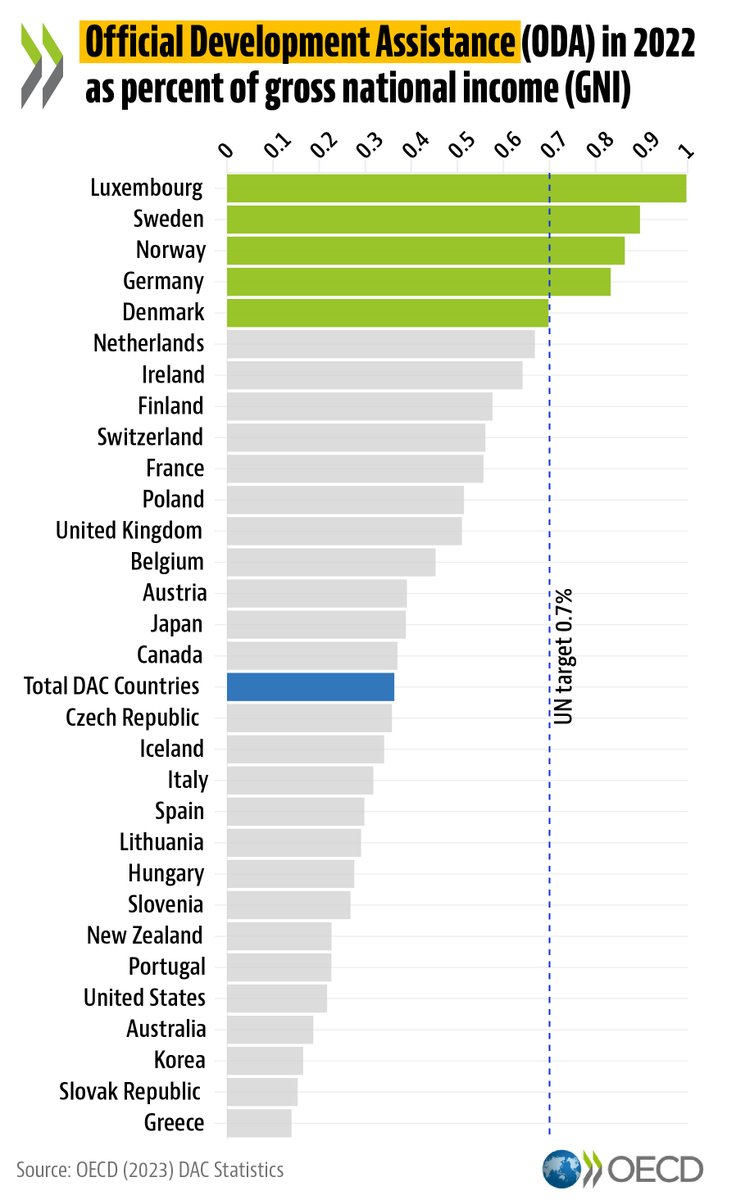
\includegraphics{figures/oecd_oda.png}

}

\caption{\href{https://twitter.com/OECDdev/status/1646419888825614336}{OECD諸国のODA/GNI比}}

\end{figure}

\hypertarget{ux56fdux969bux958bux767aux91d1ux878dux6a5fux95a2}{%
\subsubsection{国際開発金融機関}\label{ux56fdux969bux958bux767aux91d1ux878dux6a5fux95a2}}

多国間援助:\textbf{世界銀行} (World Bank: WB)
やその他の各地域の\href{https://www.mof.go.jp/policy/international_policy/mdbs/index.html}{国際開発金融機関}
(Multinational Development Bank: MDB) を通じて行う

\begin{itemize}
\tightlist
\item
  世界銀行は\href{https://www.worldbank.org/ja/about}{複数の組織}からなるグループである。

  \begin{itemize}
  \tightlist
  \item
    中核的組織は国債復興開発銀行 (International Bank Reconstruction and
    Development: IBRD) であり、戦後復興のための組織だった。
  \item
    日本の東海道新幹線もIBRDの融資によって建設
  \end{itemize}
\item
  IMFと同様に出資金の比率に応じて議決権
\end{itemize}

開発援助の一つの考えは大きな投資(\textbf{ビッグ・プッシュ})\(\leadsto\)経済成長

\begin{itemize}
\tightlist
\item
  経済成長の恩恵は次第に貧困層へと行き渡るはず(トリクル・ダウン)
\end{itemize}

資本の投下だけでは経済成長が起こらない\(\leadsto\)政治経済体制の変革

\begin{itemize}
\tightlist
\item
  新自由主義的経済政策や効率的な政府、透明性などの\textbf{グッド・ガバナンス}を援助や支援の際に求める。
\item
  IMFと世銀がワシントンで向き合って存在していることから\textbf{ワシントン・コンセンサス}と呼ばれた
\end{itemize}

\(\leadsto\)被援助国への内政干渉であり、\textbf{オーナーシップ}を尊重すべきと批判

\hypertarget{ux8ca7ux56f0ux524aux6e1b}{%
\subsubsection{貧困削減}\label{ux8ca7ux56f0ux524aux6e1b}}

冷戦終結後は貧困削減に焦点

\begin{itemize}
\tightlist
\item
  援助の限界が明らかになる/援助によって勢力を拡大する必要がなくなる
\item
  国連開発計画が\href{https://www.mofa.go.jp/mofaj/gaiko/oda/bunya/security/index.html}{\textbf{人間の安全保障}}
  (human security) や\textbf{人間開発} (human development)
  などを提唱\(\leadsto\)発展は経済だけでなく社会や個人の問題であると認知

  \begin{itemize}
  \tightlist
  \item
    人間の安全保障は日本のODA政策の中核に位置づけ
  \end{itemize}
\item
  IMFや世銀も\textbf{貧困削減ペーパー}を被援助国に作成させる
\end{itemize}

2000年に開催された国連ミレニアム・サミットの\href{https://www.mofa.go.jp/mofaj/kaidan/kiroku/s_mori/arc_00/m_summit/sengen.html}{ミレニアム宣言}\(\leadsto\)
2015年までの達成を目指して、\href{https://www.un.org/millenniumgoals/2015_MDG_Report/pdf/MDG\%202015\%20PC\%20final.pdf}{ミレニアム開発目標}
(Millennium Development Goals: MDGs) を設定

\hypertarget{ux56fdux969bux7d4cux6e08ux79e9ux5e8fux3078ux306eux6311ux6226}{%
\subsection{国際経済秩序への挑戦?}\label{ux56fdux969bux7d4cux6e08ux79e9ux5e8fux3078ux306eux6311ux6226}}

既存の国際経済秩序は先進国に有利なものであるという認識は途上国において根強い。

\begin{itemize}
\tightlist
\item
  自由貿易体制においても先進国は自国の農業を保護するために補助金やセーフガードを使用
\item
  IMFや世銀は経済規模に比例して議決権が配分されるので、先進国の意見を反映
\end{itemize}

自由な経済により先進国も途上国も互いに利益を得ることはできる/その利益の配分を巡って途上国は交渉力で先進国に対して弱い

\(\leadsto\)これまで途上国はこうした国際経済秩序の変革を目指して協力

\begin{itemize}
\tightlist
\item
  \textbf{非同盟諸国運動} (Non-Alidned Movement: NAM)
  や国連における\textbf{G77}を結成し、共同で行動
\item
  \textbf{新国際経済秩序} (New International Economic Order: NIEO)
  などを提唱
\item
  \textbf{石油輸出国機構} (Organization of the Petroleum Exporting
  Countries: OPEC) など国際カルテルによって圧力
\end{itemize}

新興国 (emerging country) 、特に中国が経済成長\(\leadsto\)大きな役割

\begin{itemize}
\tightlist
\item
  \textbf{G20}への参加、BRICS開発銀行やアジアインフラ投資銀行の設立、一帯一路の実施などで影響力
\end{itemize}

こうした新興国の経済成長は経済を自由化した結果、既存の国際経済秩序の恩恵?

民主主義による経済成長に対する反例?

\begin{itemize}
\tightlist
\item
  韓国や台湾も当初は\textbf{開発独裁}と呼ばれる、権威主義のもとでの経済成長
\end{itemize}

経済のグローバル化に対する懐疑的な見方

\begin{itemize}
\tightlist
\item
  金融危機の影響の大きさ\(\leadsto\)グローバル化の弊害。
\item
  グローバル経済への開放\(\leadsto\)期待通りの経済成長はもたらさず/国内の格差の拡大
\end{itemize}

途上国に限らず、先進国においてもグローバル化に懐疑的な政治家が登場しつつある。


  \bibliography{references.bib}


\end{document}
